\documentclass{article}


\usepackage{arxiv}

\usepackage[utf8]{inputenc} % allow utf-8 input
\usepackage[T1]{fontenc}    % use 8-bit T1 fonts
\usepackage{hyperref}       % hyperlinks
\usepackage{url}            % simple URL typesetting
\usepackage{booktabs}       % professional-quality tables
\usepackage{amsfonts}       % blackboard math symbols
\usepackage{nicefrac}       % compact symbols for 1/2, etc.
\usepackage{microtype}      % microtypography
\usepackage{lipsum}
\usepackage[ruled]{algorithm2e}
\usepackage{subcaption}

\usepackage{graphicx}
\graphicspath{ {./images/} }

\title{Training a Bipedal Robot with Deep Reinforcement Learning}


\author{
  Trey Bean \\
  Udacity Machine Learning Nanodegree\\
  Salt Lake City, UT \\
  \texttt{trey.bean@icloud.com} \\
}

\begin{document}
\maketitle

% \begin{abstract}
% \lipsum[1]
% \end{abstract}


% keywords can be removed
% \keywords{First keyword \and Second keyword \and More}


\section{Definition}
\label{sec:definition}

\subsection{Project Overview}
In the world of robotics, programming a computer-based agent to make actions by the use of a rules-based system is tedious, complex, and error-prone. In order to control the robot, programmers would directly control the specific movements, rotations, and positions of each segment and joint of the robot to complete the given task. Not only is this a cumbersome project, it is not very adaptable to handle states that weren't accounted for by the agent's designer or easy to modify it to handle different, yet similar, tasks. In the last decade or so, though, advances in machine learning and specifically deep learning, have made it possible for robotics engineers to focus less on controlling the individual components of a robot, but to instead create programs that learn how to manipulate those components to achieve a given task. While reinforcement learning has been applied to robotics in the past, the challenge of handling continuous state and action spaces made early attempts at real-world robotics challenges fail to reach much practicality. Adding deep learning to the mix, though, has allowed engineers to overcome these challenges and made the dream of things like self-driving cars and other similar-styled robots almost a reality. 

Personally, I love the problems that machine learning is allowing us to solve. However, many of those problems, e.g. spam detection, language translation, image classification, are things we interact with only through a computer or electronic devices. In order to interpret and manipulate the real-world, though, we need robots to facilitate that. I have many ideas that I wish I could build a robot for, e.g. things as simple as a dandelion-pickers to more complex robots that crawl landfills discovering recyclable and reusable material. In the past, I've known how to construct the physical robots, but have been blocked by how to program them to tackle such complex tasks. With Deep Reinforcement Learning agents, though, I'm excited to finally be able to bring some of these ideas to reality.

In this project, I will explore several leading deep learning algorithms by applying them to the task of solving a continuous state and action space environment in OpenAI's Gym, a collection of AI simulated environments that facilitates AI research, allowing researchers to compare progress against a consistent set of environments. 


\subsection{Problem Statement}
\begin{figure}[h]
\caption{Bipedal walker falling after taking random actions}
\centering
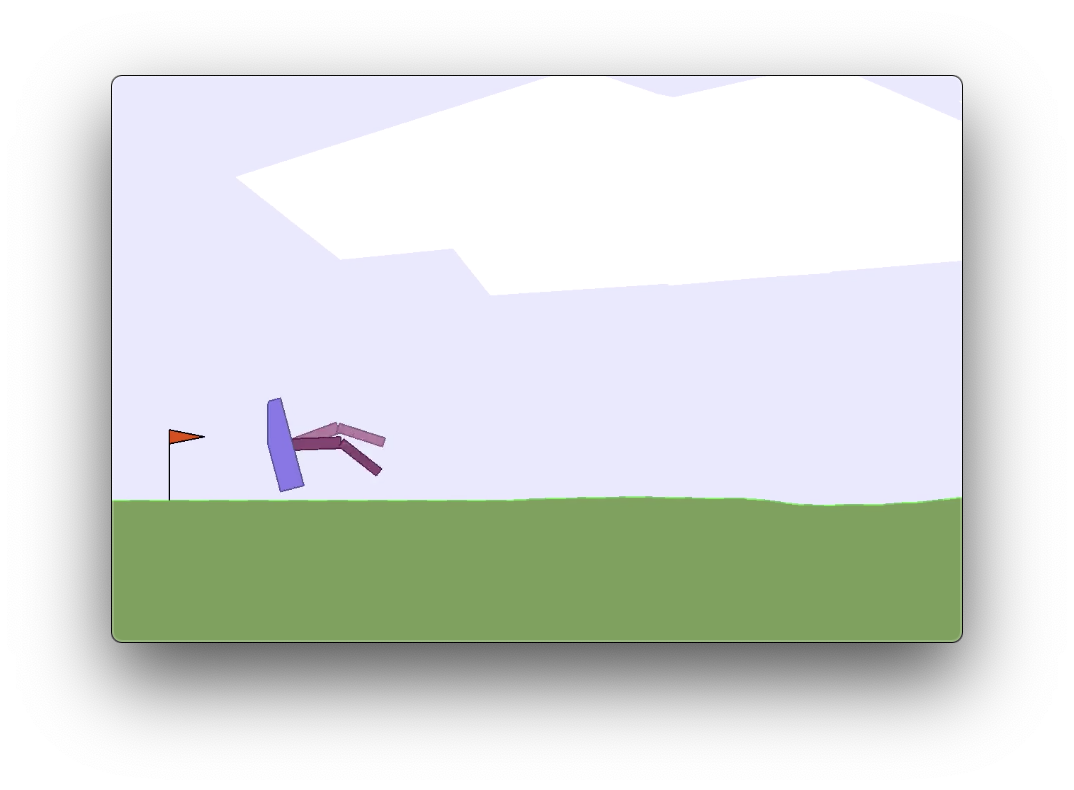
\includegraphics[scale=0.25]{images/bipedal-fall-backward.png}
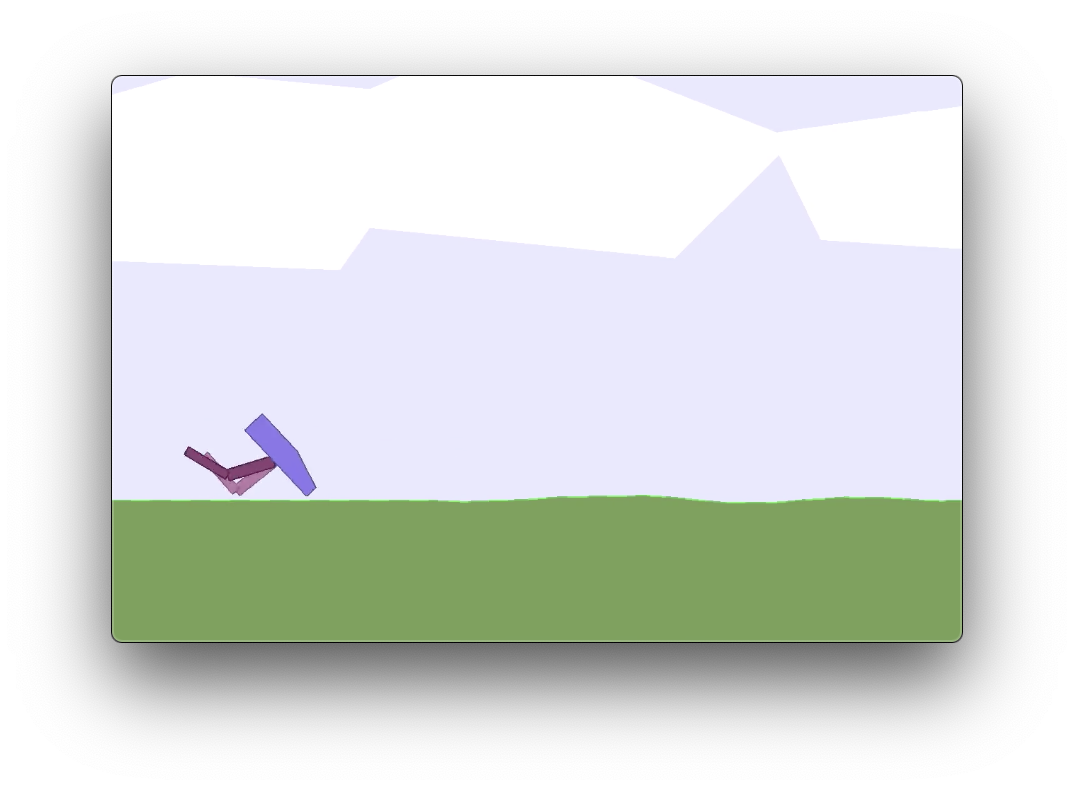
\includegraphics[scale=0.25]{images/bipedal-fall-forward.png}
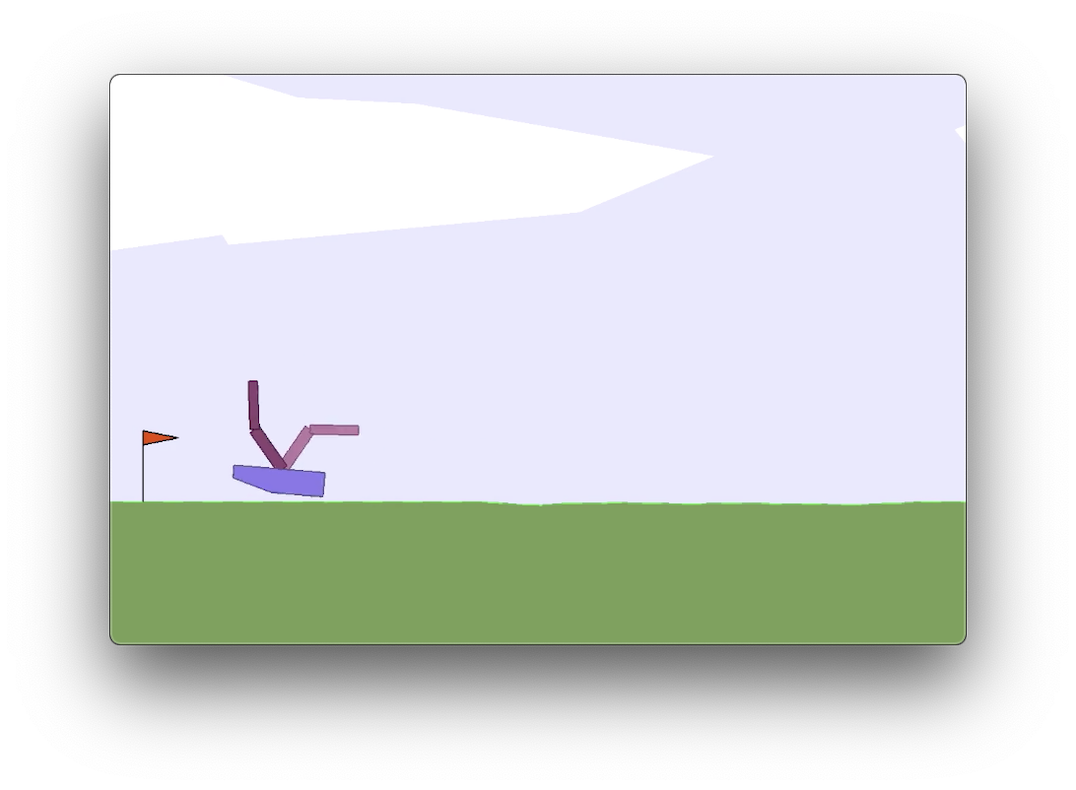
\includegraphics[scale=0.25]{images/bipedal-fall-upside-down.png}
\end{figure}

Specifically, I will be aiming to solve the BipedalWalker-v2 environment that is part of the Box2D environments on OpenAI's Gym. This environment consists of a 4-joint walker robot that is given positive reward for moving, "walking", forward. Solving is defined by OpenAI as averaging a total 300 points in 100 consecutive episodes or trials. While creating an agent that can solve the problem is the primary goal, there is a leaderboard on OpenAI that is ranked by number of episodes required before the agent solves the problem. I will compare my agent against existing results, aiming for a top result.

In order to solve this OpenAI Gym environment, which has both a continuous action and state space, I intend to first build a Deep Deterministic Policy Gradient agent (DDPG). I used this type of agent to solve the Quadcopter project—also a continuous action and state space environment—in the MLND's coursework. Additionally, I intend to explore modifications proposed in the artificial intelligence research community to reduce the tendency of DDPG agents (and other Q-learning agents) to overestimate the Q-values by building a Twin Delayed Deep Deterministic Policy Gradient agent (TD3). \cite{DBLP:journals/corr/abs-1802-09477} The TD3 agent makes the following tweaks to the original DDPG algorithm. First, instead of training only one network for Q-values, TD3 takes a page out of Double-Q Learning and trains two networks to learn two Q-functions and takes the minimum Q-value between the two to reduce value overestimation. Next, it delays updating the policy until the values of the two Q-networks have converged. Finally, this technique uses a SARSA-style update for action estimates as a regularization strategy to further reduce variance. It's my hypothesis that this TD3 agent will be less brittle and will generate a solution, on average, in fewer training episodes than the DDPG agent.

\subsection{Metrics}
Based on this challenge, there are three primary metrics I will use to evaluate and compare approaches. First, the \textbf{mean test total reward (MTTR)} achieved by the trained model. For this, I will pause learning for every episode that surpasses 200 reward points and execute the model 10 times with learning and exploration paused and use the mean episode reward returned for those episodes. While I could execute a testing path after each episode, I propose that it's a waste of time to test the model every time, especially when the episode's training pass isn't close to the goal score of 300.

Next, I will analyze the \textbf{trailing mean reward across the last 100 episodes (TMR-100)}. This will be the mean total reward across the last 100 episodes. This should tend to be slightly lower than the final trained model for that episode as it will still be learning, but it should give us a close enough comparison of trained agent performance. 

Finally, if we're able to successfully solve the environment, we will measure and compare the \textbf{number of episodes required before the agent is able to solve the problem (NES)} as defined, namely averaging a total greater than 300 points in 100 consecutive episodes.

While these are the primary metrics we'll be focusing on, we will also be logging and monitoring a secondary set of metrics, e.g. hull position, number of steps in an episode, max step reward, that should give us clues on how our agent is performing and learning.


\section{Analysis}
\label{sec:analysis}

\subsection{Data Exploration}
The data that I'll be working with in this project is generated from the OpenAI Gym environment. For the BipedalWalker-v2 environment, the state space is a 24-dimension vector of continuous attributes, all with ranges from negative infinity to infinity. These attributes correspond to the following: hull angle speed, angular velocity, horizontal speed, vertical speed, position of joints and joints angular speed, legs contact with ground, and 10 lidar rangefinder measurements. These seem like a comprehensive set of inputs to successfully train a reinforcement learning agent at the task of walking forward.  

The other key piece of data we'll be working with is the reward given at each timestep. In this environment, a reward is given for moving forward, which can total to over 300 points for reaching the far end of the environment. If the robot falls, it gets -100. Applying motor torque costs a small amount of points, thus rewarding efficient agents.

These inputs will be used to generate the next action for the robot. The action space consists of a 4-dimensional action vector that corresponds to the motor speed of each of the 4 joints. Each speed is constrained between -1 and 1. 


\subsection{Exploratory Visualization}
Because this project is a reinforcement learning problem vs. a traditional machine learning project that uses an existing dataset to train a model, there isn't as much interesting data to explore visually. That said, because the reward at each timestep is so critical to solving this environment, it is useful to see how the reward changes based on how far the BipedalWalker has progressed through the environment. Below, in figure \ref{fig:reward_v_distance}, you can see the reward—ignoring any penalty for motor torque or hull angle—plotted against the distance the BipedalWalker moved.

\begin{figure}[ht]
\caption{Plot of Reward Against Distance in the Bipedal-Walker-v2 environment}
\centering
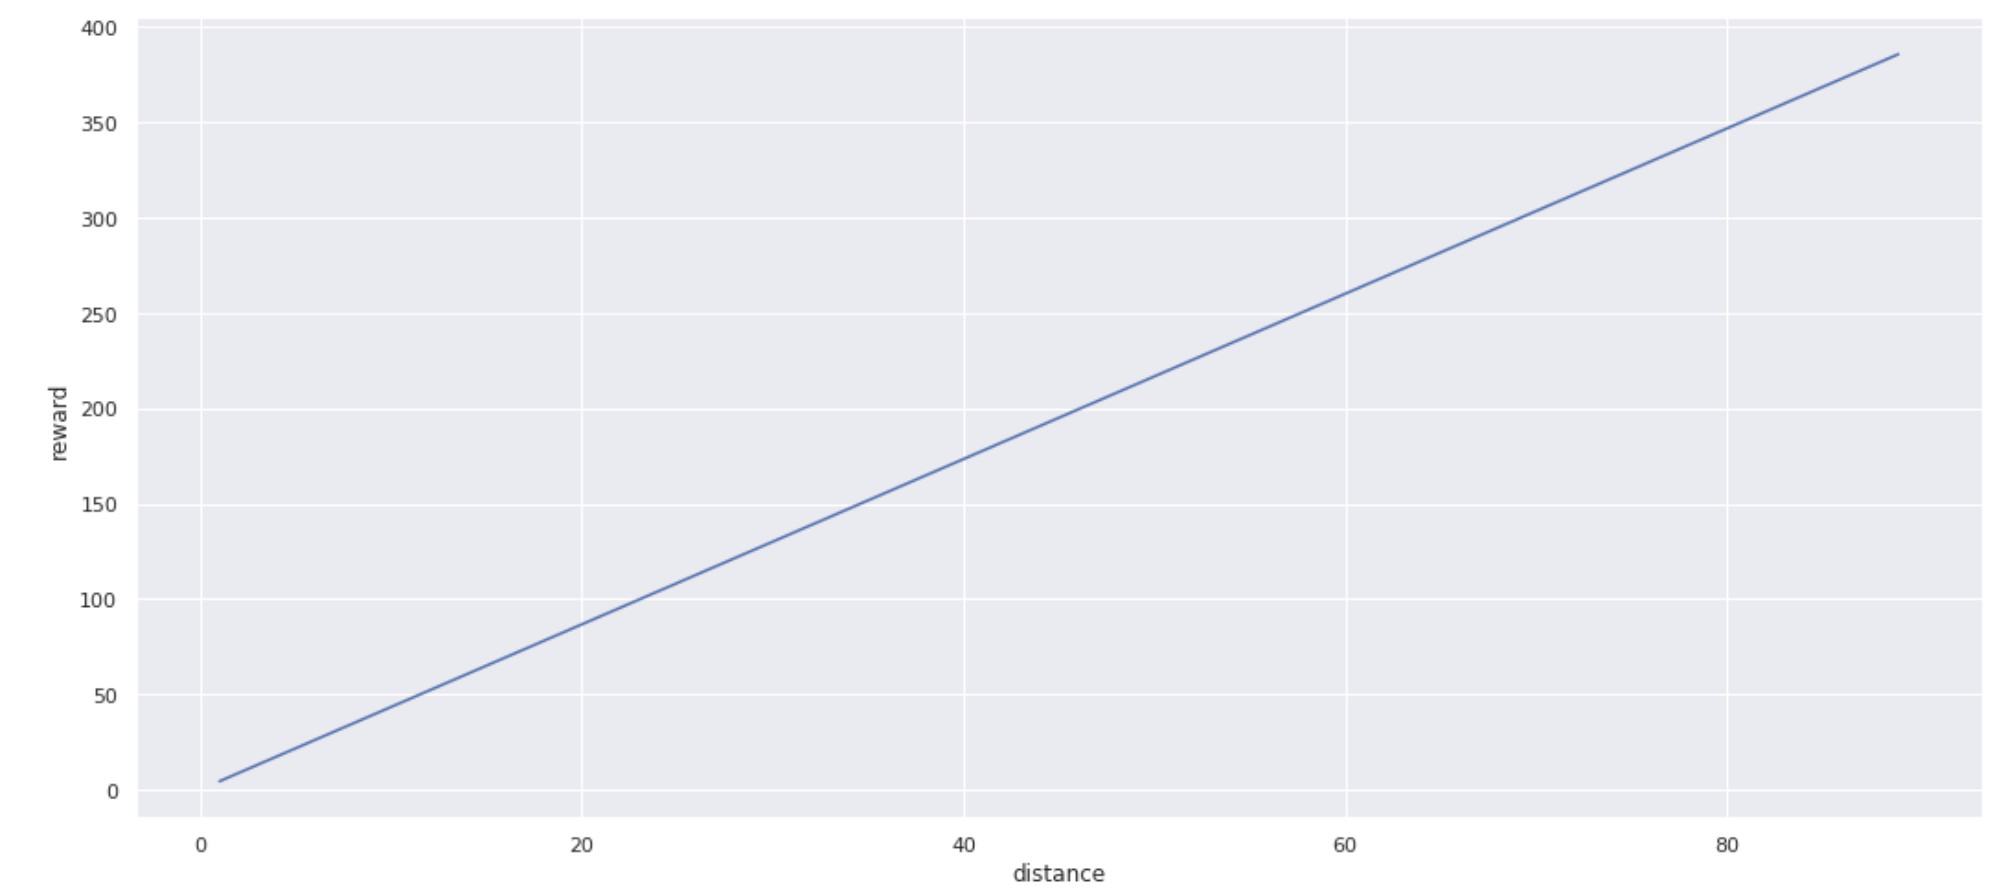
\includegraphics[scale=0.4]{images/reward_v_distance.png}
\label{fig:reward_v_distance}
\end{figure}

A couple things we should note. First, the reward increases linearly with the distance. It starts very close to zero and maxes out just below 400, based on the distance limitation in the BipedalWalker-v2 environment of 88.6. Additionally, we can see that the agent would need to travel at least 23 units in order to overcome the punishment of -100 reward for falling. Although, because the episode reward is cumulative, it


\subsection{Algorithms and Techniques}
One of the primary goals of reinforcement learning is to develop an agent that can learn a policy, or what action the agent should take given the state the agent observes itself to be in. If the environment were consistent, as in a game board, we could use approaches that aim to learn that model. This wouldn't be a good for our applications, though, because while we might be able to train a good robot that can perform in a specific configuration of the simulator, it wouldn't generalize to other environments and, given that in robotics, we'd like to use our robots in a multitude of diverse environments, we'd instead like to arrive at a solution that is able to generalize, so we'll use model-free approaches. 

In terms of model-free reinforcement learning techniques, there are two main categories of techniques: policy optimization and q-learning. In policy optimization, the agent attempts to an optimal policy that maximizes the reward. This is nice because it's ultimately what we want our agent to do. Unfortunately, policy optimization techniques are very slow and are very susceptible to getting stuck in a local optima. Another approach, Q-learning, attempts to learn an action-value function, $Q_{\theta}(s, a)$, which approximates the value of taking an action, given a current state. A policy can then be specified for taking the action that yields the maximum value. While now only indirectly optimizing for the performance of the agent, Q-learning techniques tend to be much more efficient in reusing data. That said, they tend to be far less stable than policy-optimization techniques. 

Luckily for us, there are approaches that combine both approaches, like Deep Deterministic Policy Gradients (DDPG), Twin Delayed Deep Deterministic Policy Gradient (TD3), and Soft Actor-Critic. All of these techniques, at a high-level, follow the actor-critic methodology, of learning "approximations to both policy and value functions ..., where ‘actor’ is a reference to the learned policy, and ‘critic’ refers to the learned value function, usually a state-value function" \cite{Sutton:2018:RLI:3312046}. 

For this project, I will implement the DDPG algorithm and ideally solve the underlying OpenAI BipedalWalker-v2 environment. This method works by learning both a policy and a Q-function at the same time. As the agent explores the environment, trying to learn the policy, it stores the state, action, reward data in a replay buffer. The "critic" uses this data, off policy (because the data no longer corresponds to the most recently updated policy), to learn the Q-function using deep learning networks, optimizing by minimizing the Bellman error. The "actor", then uses this Q-function to learn the optimal policy through gradient ascent, also through a deep learning networks. It's worth pointing out that because Q-learning is trying to minimize the MSBE loss, the target network depends on the same parameters. To reduce the instability this results in, we delay updating the target network. In DDPG, the target network is updated once per main network update using poyak averaging.

After implementing the DDPG algorithm successfully, I will explore building a Twin Delayed Deep Deterministic Policy Gradient agent (TD3). The TD3 agent makes the following tweaks to the original DDPG algorithm. First, instead of training only one network for Q-values, TD3 takes a page out of Double-Q Learning and trains two networks to learn two Q-functions and takes the minimum Q-value between the two to reduce value overestimation. Next, it delays updating the policy until the values of the two Q-networks have converged. Finally, this technique uses a SARSA-style update for action estimates as a regularization strategy to further reduce variance. It's my hypothesis that this TD3 agent will be less brittle and will generate a solution, on average, in fewer training episodes than the DDPG agent.

At this point, I will compare the performance of TD3 and DDPG in solving the BipedalWalker-v2 environment, specifically comparing the number of episodes required before the agent is able to solve the problem as defined, assuming both agents are able to solve the environment.

Additionally, based on some ideas in the both of the papers about these algorithms and my experience on the Quadcopter project, I intend to explore different noise strategies as well as different sizes for the hidden layers to measure the impact on these attributes of the agents.


\subsection{Benchmark}
As a benchmark model, I elected to use a Vanilla Policy Gradient (VPG) algorithm. The VPG algorithm is a model-free, on-policy algorithm that uses gradient ascent to optimize policy performance. In many ways, it's very similar to the actor portion of the DDPG and TD3 algorithms, but instead of training on the Q-function learned by the critic, it learns by sampling actions given its current policy and updates that policy using stochastic gradient ascent.

For the benchmark run, I ran the VPG agent implemented by OpenAI on the Bipedal-Walker-v2 environment using OpenAI's Spinning Up experiment runner for 1000 epochs at 4800 steps per epoch and a maximum episode length of 1600. The gamma was set to 0.999. The rest of the configuration used default values for the experiment runner and VPG algorithm. As you can see in Figure \ref{fig:benchmark_results}, this model was able to learn the environment and increasingly perform better, but it wasn't able to "solve" the environment by scoring over 300 points in 100 consecutive episodes. Specifically, after running 3000 episodes (1000 epochs), the TMR-100—in this case, the average total reward given over the last 99 episodes (33 epochs), since the experiment runner doesn't report results for each episode—was 89.91. And you can see from the chart that the agent still falls and gets penalized the -100 points. 

\begin{figure}[ht]
\caption{Plot of Average Total Reward per Episode for Vanilla Policy Gradient algorithm on the Bipedal-Walker-v2 environment}
\centering
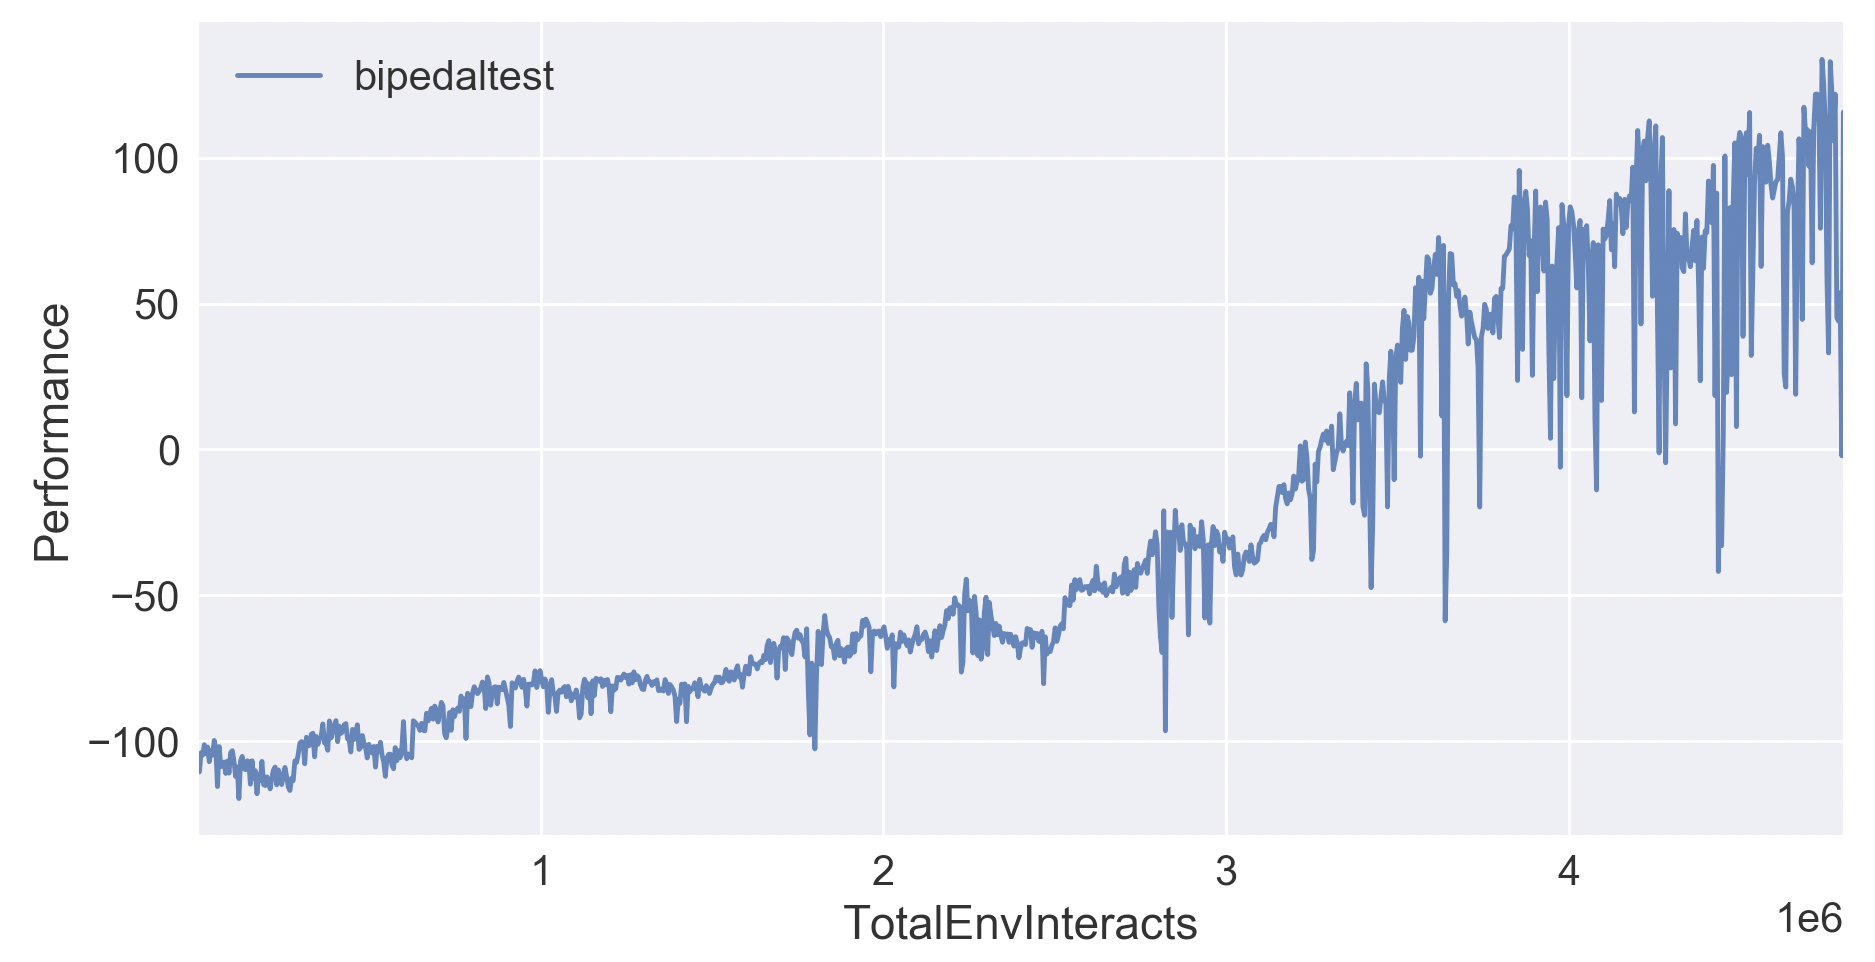
\includegraphics[scale=0.4]{images/bipedal-vpg-performance-plot.png}
\label{fig:benchmark_results}
\end{figure}


\section{Methodology}
\label{sec:methodology}

\subsection{Data Preprocessing}
Because this is a reinforcement learning project where the "data" is "observed" from the OpenAI environment and not a standard machine learning project starting with an existing dataset, there really isn't any "preprocessing" to be done. The only choice I really had to make was whether to constrain the potential actions beyond what the environment allows, e.g. if I didn't want to allow the agent to make actions near the extremes of the action space or to constrain them relative to each other. I chose not to do this because when I explored applying techniques like this in the Quadcopter project in the MLND coursework, it didn't yield positive results and instead it was better for the agent to "learn" those.


\subsection{Implementation}
Since I knew my plan was to be able to compare both and DDPG and TD3 agent, I began by implementing a primary function that would interface with either agent. This primary function defined in \textit{main.py} controlled which agent to train and test against, how many episodes to train on, when to pause training to execute the testing of the trained agent, and a normalized results structure for capturing the same metrics regardless of agent being trained. This last part ensured that I was recording and comparing metrics collected in exactly the same manner. 

The basic algorithm for primary function is this:

\begin{algorithm}[H]
\SetAlgoLined

initialize training settings\;

\For{$i=0$ \KwTo $episodeCount$}{
    $episodeReward \longleftarrow 0$\;
    reset agent and environment\;
    
    \For{$t=0$ \KwTo $maxEpisodeLength$}{
        $action \longleftarrow agent.getAction(observation)$\;
        $nextObservation, reward, done, info \longleftarrow env.step(action)$\;
        $episodeReward \longleftarrow episodeReward + reward$\;
        $agent.step(observation, action, reward, nextObservation, done)$\;
        $observation \longleftarrow nextObservation$\;
        
        \If{$done$}{
            record metrics\;
            \If{$episodeReward > 200$}{
                test agent\;
            }
        }
    }
}

close environment and output files\;

\caption{Primary Agent Training Algorithm}
\end{algorithm}

This algorithm can then be used to train and test any agent that implements the necessary functions. 

Once this framework was in place, I implemented the Deep Deterministic Policy Gradient algorithm using Python and Keras. As described above, I used the same architecture and hyperparameters as described in the original paper about this technique \cite{DBLP:journals/corr/LillicrapHPHETS15}. It uses two hidden layers for each network, a 400 and 300 unit dense layer. For the actor, I used a tanh activation layer. I initialized the final layer weights and biases of both the actor and critic networks from a uniform distribution between $-3e^{-3}$ and $3e^{-3}$ to ensure the initial outputs for the policy and value estimates are near zero. I used a $10^{-4}$ and $10^{-3}$ learning rate for the actor and critic networks respectively. I used Adam optimization for both networks. I used a $\gamma$ of 0.99 and a $\tau$ of 0.001. For the critic network, I employed L2 weight decay of $10^{-2}$. Finally, I used the Ornstein-Uhlenbeck process with $\theta = 0.15$ and $\sigma = 0.2$ for the exploration noise process. I used a batch size of 64 and a replay buffer size of $10^{6}$. 

I went through many iterations with the basic DDPG algorithm, experimenting with various network architectures and configurations. I was frustrated that while it was learning, as could be seen with decreasing losses and increasing rewards, I felt like it should be able to be trained faster. Further, I wasn't able to get the agent to fully solve the environment. It learned, and by outputting video of the agent, I could see that the walker was walking to the end of the environment, but it still occasionally fell and I wasn't able to get it to hit the success criteria of averaging over 300 for 100 consecutive episodes after training for 20,000 episodes.

After weeks of experimentation, I began to feel like the DDPG had hit a limit on this problem and either I would need to explore different architectures for the actor and critic networks, use a different set of hyperparameters, or train the agent for a lot longer (or some combination of the three) in order to officially solve the problem. I decided to implement the TD3 algorithm and see how it compared. 

The Twin Delayed Deep Deterministic Policy Gradient agent (TD3) algorithm is primarily a set of improvements aimed at improving the performance of the DDPG algorithm. Specifically, it aims to address "overestimation bias and the accumulation of error in temporal difference methods" by training two networks to learn two Q-functions and using the minimum Q-value between the two to reduce value overestimation; delaying updating the policy until the values of the two Q-networks have converged; and using a SARSA-style update for action estimates as a regularization strategy to further reduce variance \cite{DBLP:journals/corr/abs-1802-09477}. 

In order to implement the TD3 algorithm, I copied the working DDPG code into a new agent that could be fed into our primary training function. I then duplicated the Q-network of the critic, using the same parameters for both networks. I then modified the agent to use the minimum Q-value from the critic networks to reduce value overestimation. Next, I added a condition to only update the policy every other iteration instead of every iteration as is done in the DDPG algorithm. Finally, I implemented the target policy smoothing regularization technique, by adding a clipped amount of noise during the target policy update with a modified target update: $y=r+\gamma Q_{\theta'} (s', \pi_{\phi'}(s')+ \epsilon)$, where $\epsilon \sim clip(\mathcal{N}(0, \sigma), -c, c)$.

With the addition of the extra Q-value network, I had to update the primary function to allow for tracking Q-loss metrics for both Q-value networks. With these tweaks in place, I was able to successfully train the TD3 agent on the BipedalWalker-v2 environment. While it didn't fully solve the environment to the specific success criteria defined by OpenAI, it outperformed the DDPG agent in two ways. It had a higher max TMR-100 of 253 vs. the -8 of the DDPG's max TMR-100. Further, it reached it's best MTTR of 284 after 4,262 training episodes compared to DDPG's best MTTR of 270 after episode 19,709.


\subsection{Refinement}
During the weeks of trying to get the DDPG agent to successfully learn the environment, I tried many, many things. First, I started with the same network architectures and hyperparamters I used in the Quadcopter project. This used a simpler network architectures from those outlined in the original DDPG paper, with two hidden layers for each networks, a 32 and 64 unit dense layers. It also used Batch Normalization layers L2 regularizers between each hidden layer. My theory was that it might be faster for the algorithm to converge on a solution than using the larger networks outlined in the DDPG paper, even if the solution wasn't as ideal. As you can see in Figure \ref{fig:ddpg_refinement}, this model failed to show any learning after 1000 episodes.

\begin{figure}[ht]
\caption{Plot of Episode Reward across 1000 episodes between initial DDPG agent and final DDPG agent}
\centering
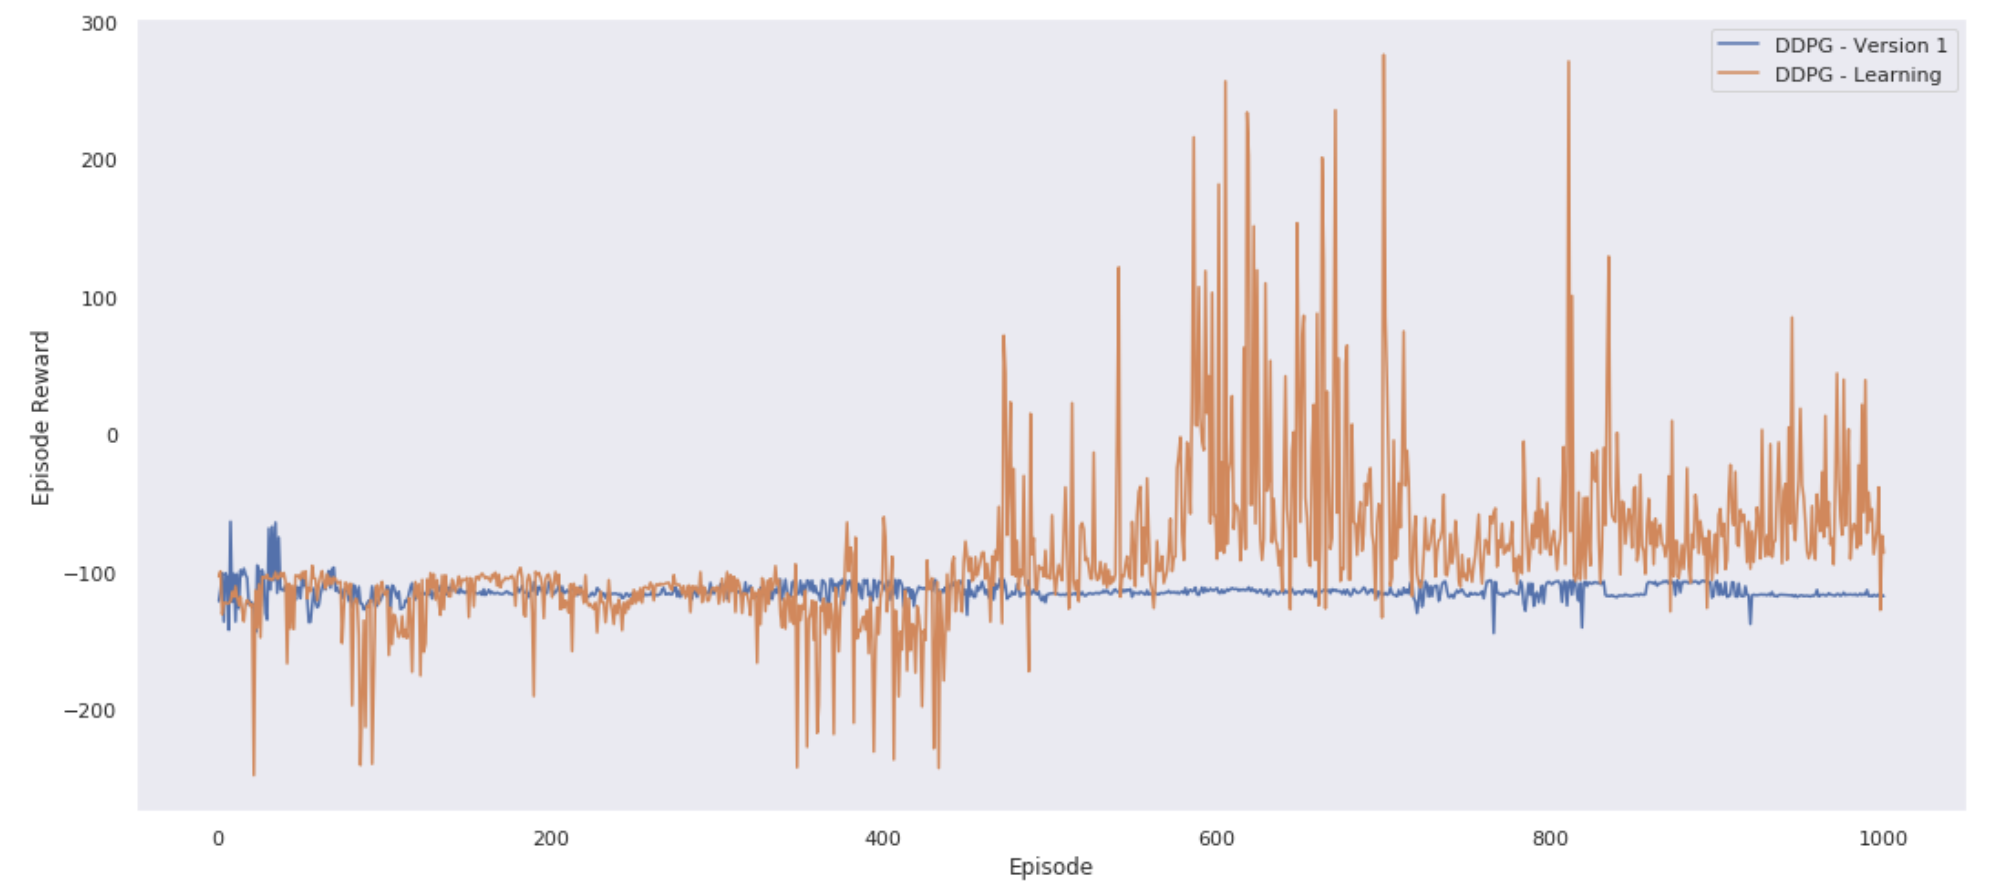
\includegraphics[scale=0.4]{report/images/ddpg_refinement.png}
\label{fig:ddpg_refinement}
\end{figure}

I then switched to using the 400, 300 layer densities outlined in the papers, removed the Batch Normalization layers, and removed the manual scaling of the actions that was done in the Quadcopter code. Instead I used a final $tanh$ activation layer, since the output of $tanh$ is [-1, 1], matching our action ranges. Finally, and I think this was my biggest breakthrough, I removed the kernel regularizer that I was applying to each layer in my networks in both the actor and critic. It's my belief that the way that I was doing this was not the way to apply the batch normalization L2 weight decay outlined in the DDPG paper. Once I removed that, I began getting progressively lower losses and eventual learning yielding the results outlined above. 

Another path of refinement that I explored, but didn't ultimately use, was the buffer size of the replay memory. The original DDPG paper used a buffer size of $10^{6}$. As I was watching my agent seem to start to learn and have periods of high rewards only then drop back to failing quickly, I surmised that one cause could be that the successful state/action pairs getting stored in the replay buffer were getting flushed from the replay memory too quickly, possibly because this environment had a larger state and action space. I experimented increasing this to $10^{7}$ and $10^{9}$, but didn't observe any significant improvements.


\section{Results}
\label{sec:results}

\subsection{Model Evaluation and Validation}

\begin{figure}[h]
\caption{Training Episode Rewards received in both DDPG and TD3 agents}
\centering

\begin{minipage}[t]{.5\linewidth}
\centering
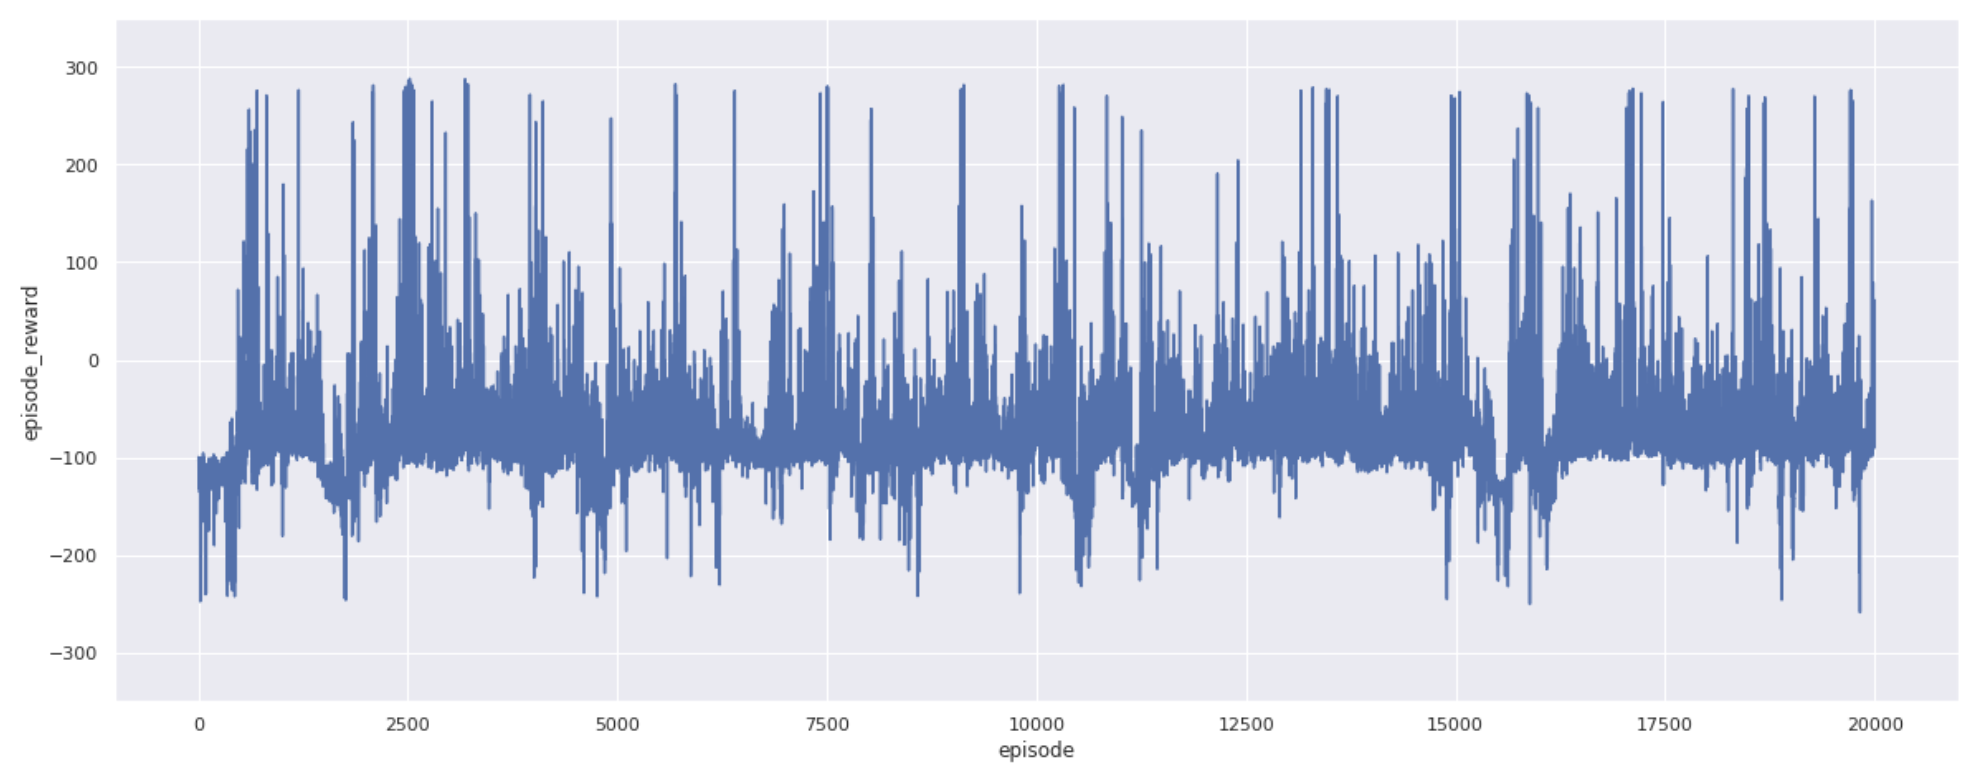
\includegraphics[width=\linewidth, height=4cm]{images/episode_reward_ddpg.png}
\subcaption{DDPG}\label{fig:a}
\end{minipage}%
\begin{minipage}[t]{.5\linewidth}
\centering
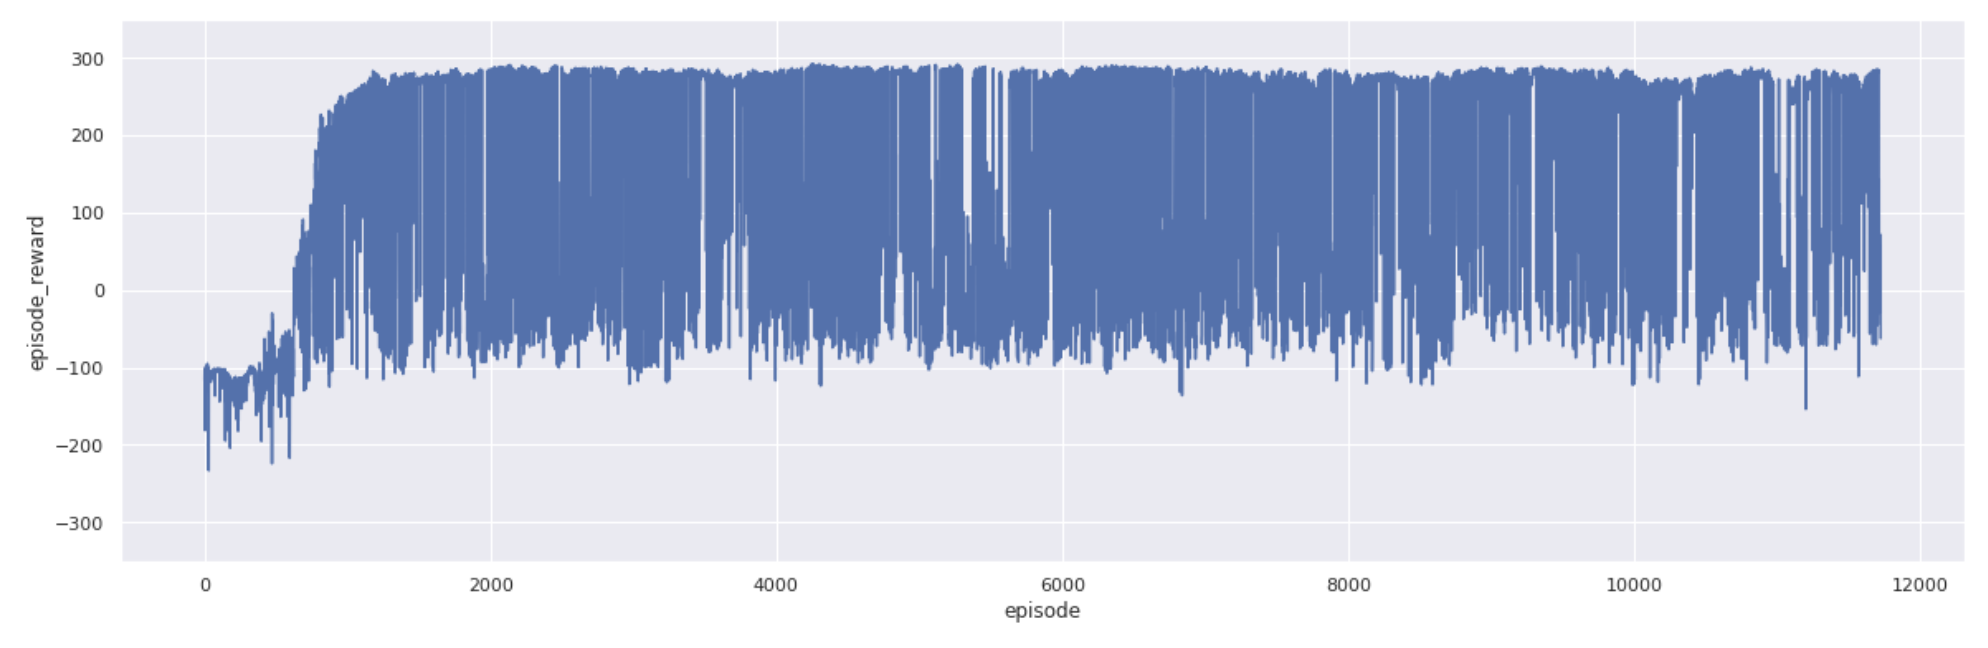
\includegraphics[width=\linewidth, height=4cm]{images/episode_reward_td3.png}
\subcaption{TD3}\label{fig:b}
\end{minipage}
\label{fig:episode_rewards_results}
\end{figure}


\begin{figure}[h]
\caption{Mean Test Total Reward (MTTR) received in both DDPG and TD3 agents}
\centering

\begin{minipage}[t]{.5\linewidth}
\centering
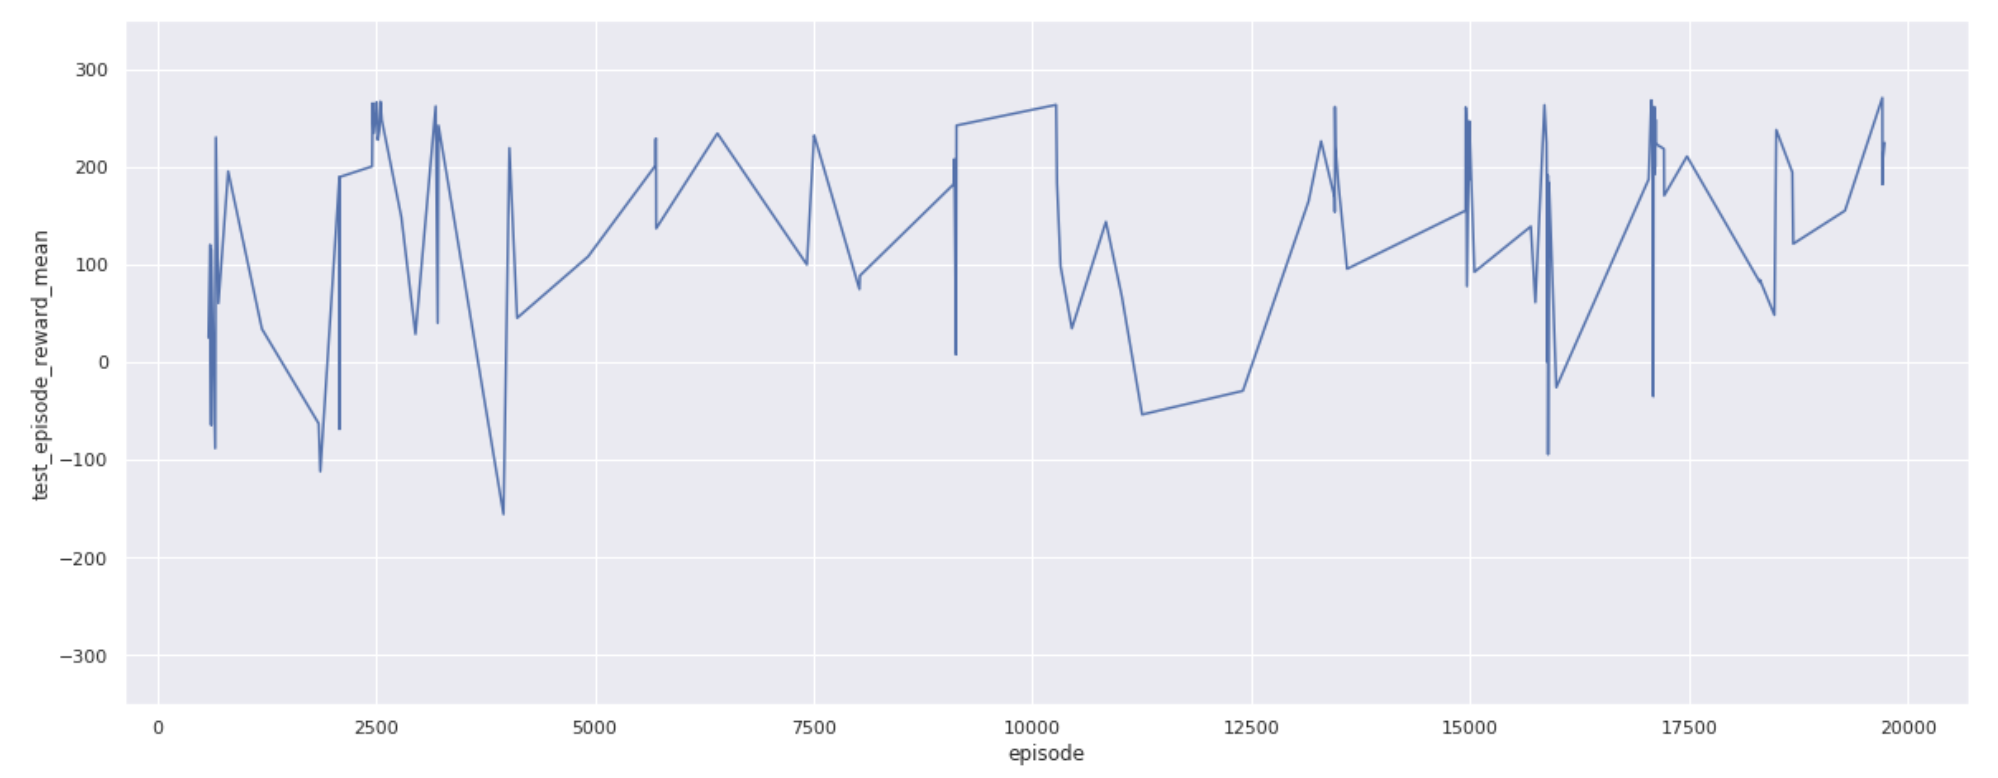
\includegraphics[width=\linewidth, height=4cm]{images/test_episode_reward_mean_ddpg.png}
\subcaption{DDPG}\label{fig:a}
\end{minipage}%
\begin{minipage}[t]{.5\linewidth}
\centering
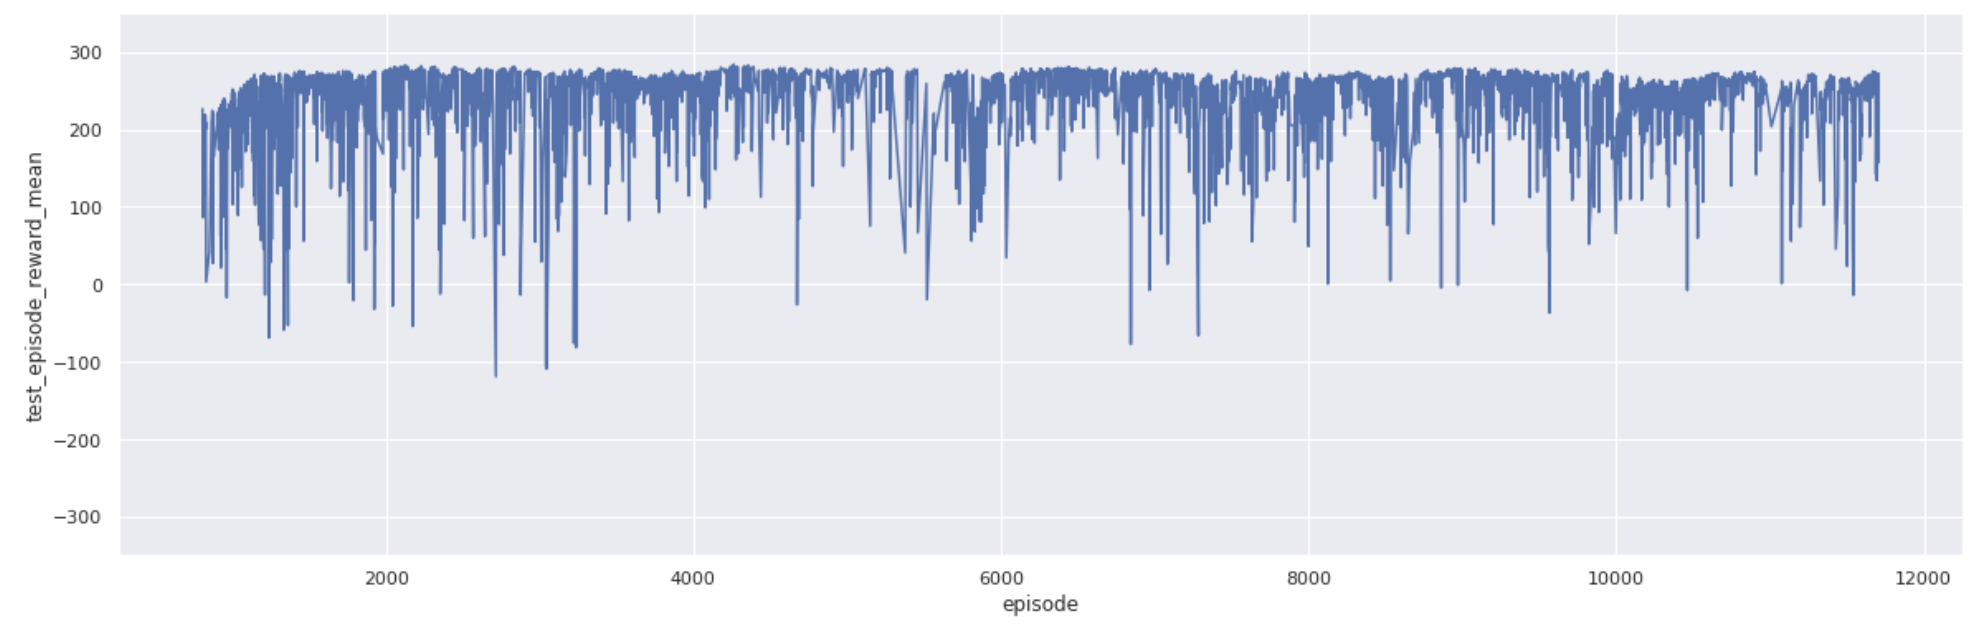
\includegraphics[width=\linewidth, height=4cm]{images/test_episode_reward_mean_td3.png}
\subcaption{TD3}\label{fig:b}
\end{minipage}

\label{fig:mttr_results}
\end{figure}

Between the benchmark Vanilla Policy Gradient (VPG), the Deep Deterministic Policy Gradient (DDPG), and the Twin Delayed Deep Deterministic Policy Gradient (TD3) agents, I feel like the performance of the TD3 agent, both in receiving a higher reward and in reaching a best solution faster, makes it the best algorithm/model to use for this project.

As you can see in Figure \ref{fig:episode_rewards_results}, the episode reward is very erratic in the DDPG agent. Because of this, it doesn't hit the condition, of receiving greater than 200 in an episode, to run a test as often as in the TD3, 112 times vs. 6,031 as can be seen in Figure \ref{fig:mttr_results}.

You can see in \ref{fig:episode_rewards_results} that both agents demonstrate the characteristic curve of a learning agent. In one of the only areas that the DDPG seems to outperform TD3 was in speed of initial learning. The DDPG agent was able to reach the condition that kicks off a test round after 586 episodes, compared to the 807 required by the TD3 agent. 

In order to validate the model, as already described above, once an episode produced a reward of greater than 200, we initiated a test sequence which stopped training and ran the agent through a new environment 10 times, recording it's minimum, maximum, and mean reward for the 10 test runs. Further, for any model that reached this stage, I saved the weights for all of the networks in both the actor and critic. This allowed me to load the weights for that episode and run the saved agent through the environment as many times as I wanted as well as to use the video capabilities in OpenAI to visualize exactly how the agent was performing. 


\subsection{Justification}
We've compared the performance of the DDPG and TD3 agents, but how do the perform compared to the benchmark VPG agent? 

\begin{figure}[h]
\caption{Benchmark vs. TD3}
\centering
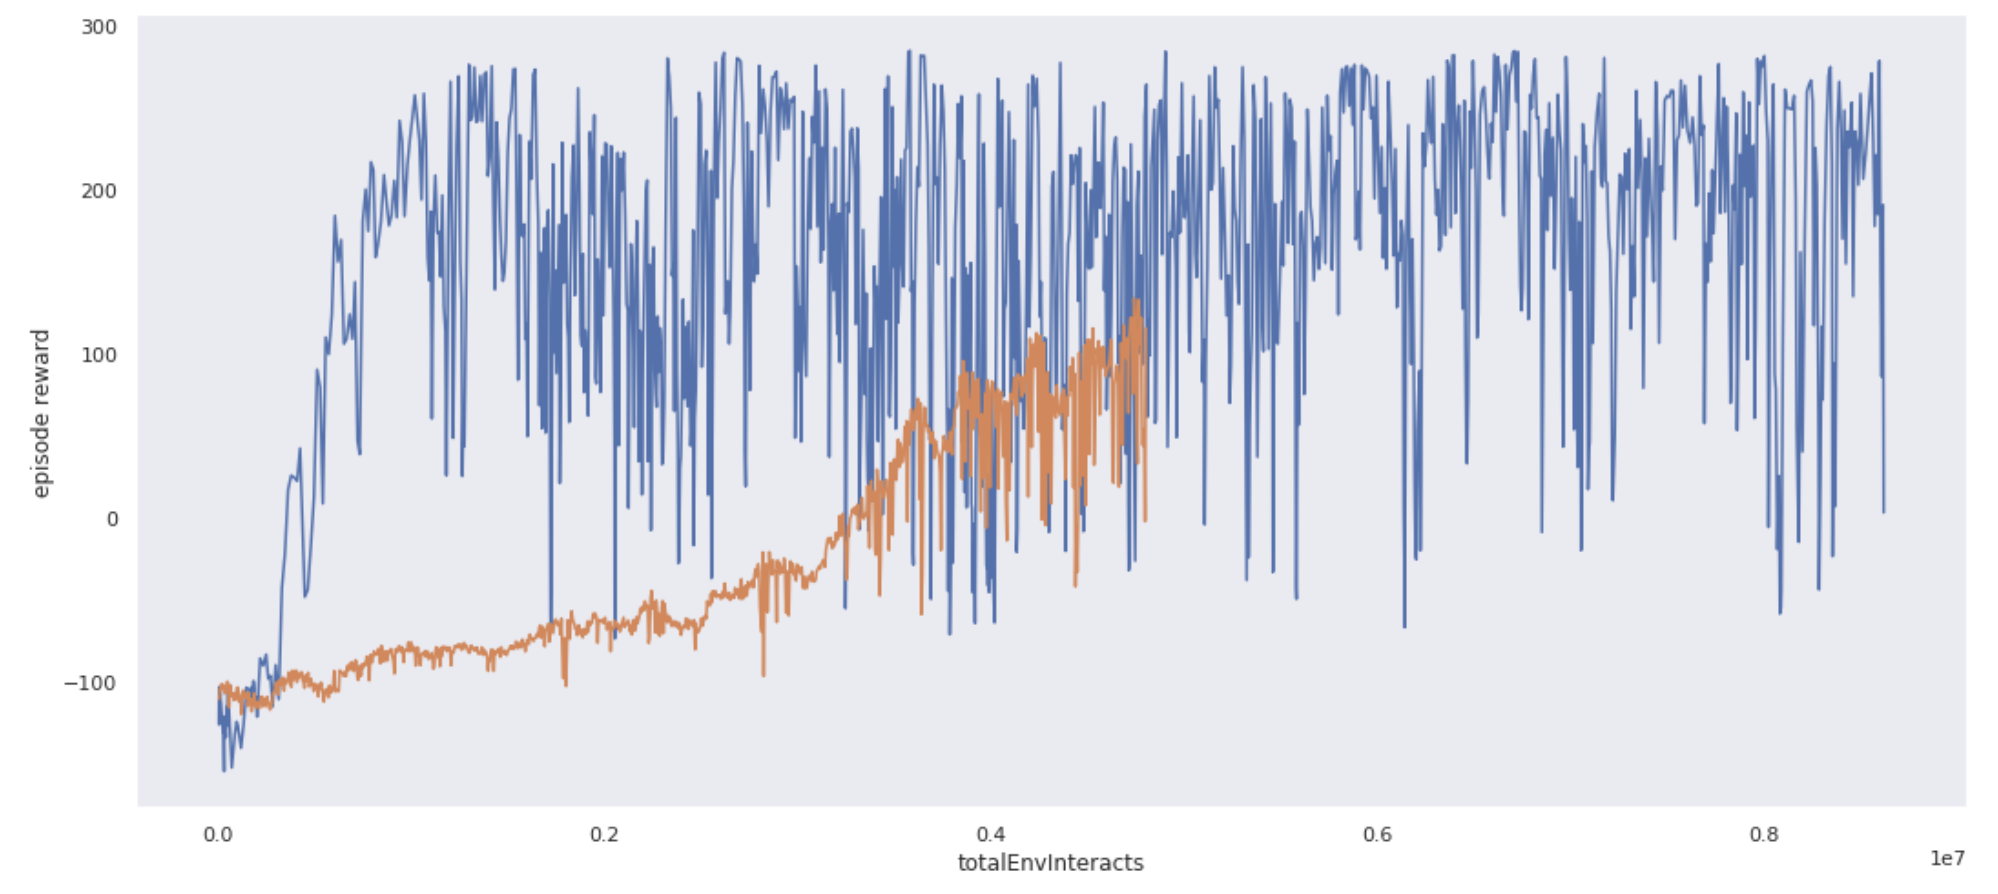
\includegraphics[scale=0.4]{images/benchmark_v_td3.png}
\label{fig:benchmark_v_td3}
\end{figure}

As you can see in \ref{fig:benchmark_v_td3}, in order to mimic the same visualization that was used by the OpenAI SpinningUp runner, I grouped the episodes from the TD3 results into epochs of 10 episodes and calculated the cumulative time steps at each epoch, which SpinningUp labelled as "TotalEnvInteracts". From this chart, you can clearly see that the TD3 agent learns much quicker than the benchmark VPG algorithm. 

It's important to note, though, that I stopped the benchmark run after 100 epochs, which resulted in 4.8M steps. When running the TD3 and DDPG agents, I was increased the max episodes to 20,000 to see if it would ever reach a full solution to the OpenAI environment. This led to more steps, or interactions with the environment, 8.6M, in the TD3 environment. 

Clearly, the TD3 agent outperforms the VPG agent in terms of time to learn and total average reward. That said, there are some compelling characteristics of the VPG agent. It's far less brittle and erratic than the TD3. I imagine this is because of the random sampling from the replay buffer that the TD3 agent uses to learn. 

While we didn't fully solve the environment to OpenAI's specification, and especially after watching the videos of the agent performing, I feel like this is an acceptable final solution as the agent does walk to the end of the environment. It just doesn't get the maximum reward becasue it's not taking the most efficient actions. I imagine through further training, we could get it there.


\section{Conclusion}
\label{sec:conclusion}

\subsection{Free-Form Visualization}
While we looked at some visualizations of important metrics in the previous sections, I feel like it's important to also see the actual progress of the trained agent in terms of the actual goal of the environment, namely to walk forward across the environment. As part of my debugging process, I began logging how far the agent made it before the episode ended, through either the time expiring, the robot falling, or it reaching the furthest edge of the simulated environment. Below, in Figure \ref{fig:hull_positions}, you can see the plot of distances reached by both DDPG and TD3.

\begin{figure}[h]
\caption{Hull x position at the end of each episode for both DDPG and TD3, with linear regression line (order=3) shown. Episodes are binned by 1000.}
\centering

\begin{minipage}[t]{.5\linewidth}
\centering
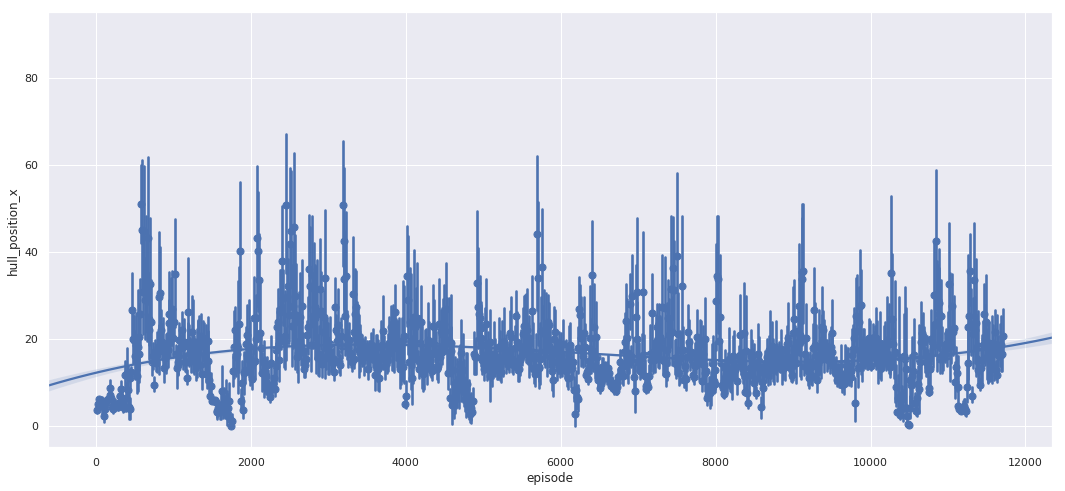
\includegraphics[width=\linewidth, height=4cm]{images/hull_position_x_ddpg.png}
\subcaption{DDPG}\label{fig:a}
\end{minipage}%
\begin{minipage}[t]{.5\linewidth}
\centering
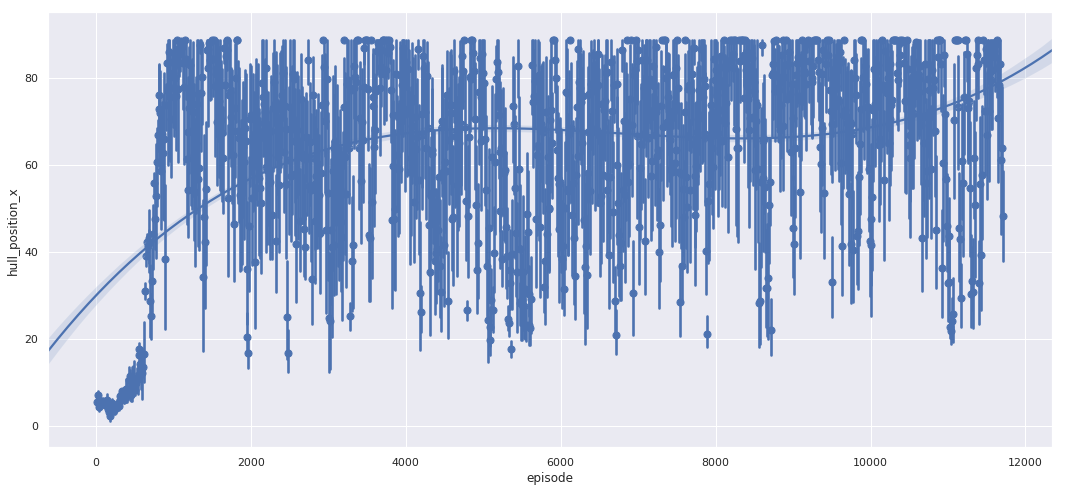
\includegraphics[width=\linewidth, height=4cm]{images/hull_position_x_td3.png}
\subcaption{TD3}\label{fig:b}
\end{minipage}
\label{fig:hull_positions}
\end{figure}

In some ways, this is one of the better illustrations of how the TD3 agent easily outperforms the DDPG agent. While you can see that the DDPG agent does learn to walk, it never gets to the edge of the environment and, as discussed above, quickly seems to forget it's progress and returns to falling pretty quickly or walking slowly, but on average only makes it 17.01 distance units vs. the 63.6 distance units the TD3 agent travels on average.

It's interesting to note the maximum bound shown in the TD3 chart too. For a while, I couldn't figure out why an episode that accumulated a high score, e.g. above 200, would not use all of the 1600 timesteps allotted and would end early. I had to go into OpenAI's code to discover that they explicitly call game over if the agent reaches a maximum distance. This is when I concluded that the TD3 agent had actually done a far superior job of solving the environment, but just hadn't figured out how to do it in an efficient, and slow?, enough way to average over 300 points over 100 test episodes. 


\subsection{Reflection}
In this project, I was able to successfully tackle a the very difficult problem or programming a 4-joint bipedal walker robot to navigate an environment without using antiquated rule-based methods. Instead, the agent learned through successive training episodes what good actions it should take for any given state the robot observes itself being in. I was able to achieve this by utilizing two actor-critic algorithms, a Deep Deterministic Policy Gradient (DDPG) and a Twin Delayed Delayed Deep Deterministic Policy Gradient (TD3). By reading works on reinforcement learning agents in continuous action and state spaces, it was clear these two methods were worth exploring. I first implemented the DDPG based on the work I did in the Quadcopter project in the MLND coursework. The first stab was using a simpler network architecture than was prescribed in the DDPG paper, so after a lot of experimentation, I implemented that approach in Keras as best as I could. This resulted in an agent that learned the environment and produced some decently trained models, but not one that was good enough to solve the environment fully based on the success criteria specified by OpenAI. I then implemented the TD3 modifications outlined in that paper. This resulted in an agent that, while training a bit slower, clearly outperformed the DDPG agent in both performance and consistency. Unfortunately, this too wasn't able to fully solve the OpenAI environment like I had hoped, but it did result in a robot that could successfully walk to the edge of the environment on a majority of episodes, so I still felt pretty awesome when I compared it to what I thought was possible in robotics programming prior to this course. I'm excited to continue to apply techniques like this in the general setting of other similar robotics problems with continuous action and state spaces.

The most interesting aspects of this project were easily watching the logs as the agent was learning—it's so gratifying when losses start decreasing and the rewards start increasing!!! And by no means was this an easy project. Designing and tuning a deep-learning reinforcement agent to a particular environment proved very tricky, especially given the long feedback cycle. 


\subsection{Improvement}
As with many projects, time is finite and you have to submit before you're fully satisfied. The same is true here. I plan on continuing to explore my implementation of the TD3 algorithm to try and tune it and achieve greater performance. For example, the batch normalization layers I had inserted to match the algorithm as described in the paper didn't seem to be working as expected, so I removed them from my final TD3 implementation. From what I've read, adding them back in should improve results, at least in converging on a solution faster. Additionally, the paper described combining the states and actions immediately as opposed to after the second dense layer as was done by the original DDPG team. When I tried this, I wasn't able to get the agent to learn, so I intend to spend more time on figuring out how to do that in Keras as I expect that to speed up training.

Finally, if I'm not able to achieve a true, full solution to the environment using TD3, I've read about genetic algorithms and evolution strategies that seem promising for problems like this and even if they don't perform better, they seem interesting enough that I want to try them out to see how they compare to a deep-learning, actor-critic approach.

Ultimately, I have read about others who have achieved better results, so I know a better solution exists and I intend to continue to discover how to improve my implementation to at least match their results.

\bibliographystyle{unsrt}  
\bibliography{references}

\end{document}
